In this chapter, we apply MCMC algorithm to learn synchronous graph grammars for mapping strings
to graphs structure. Specifically, we learn Synchronous Hyperedge Replacement Grammar (SHRG) rules from a forest that represents likely derivations consistent with a fixed string-to-graph 
alignment. We make an analogy of string-to-AMR parsing to the task of phrase-based machine translation and
come up with an efficient algorithm to learn graph grammars from string-graph pairs. We present our existing framework and propose some new techniques with specific motivations that have
be helpful to improve our existing pipeline.
\section{Introduction} 
Abstract Meaning Representation (AMR) \cite{banarescu2013abstract} is a semantic formalism where the meaning 
of a sentence is encoded as a rooted, directed graph. 
Figure~\ref{fig:amr-example} shows an example of the edge-labeled representation of an AMR 
graph where the edges are labeled while the nodes are not. The label of the leaf edge going out of a node represents 
the concept of the node, and the label of a non-leaf edge shows the relation between the concepts of the two nodes it connects to. 
This formalism is based on propositional logic and neo-Davidsonian event representations~\cite{parsons1990events,Davidson:1967}.
AMR does not encode quantifiers, tense and modality, but it jointly encodes a set of selected semantic phenomena which renders
it useful in applications like question answering and semantics-based machine translation.

\begin{figure}
\begin{center}
\scalebox{0.50}{
    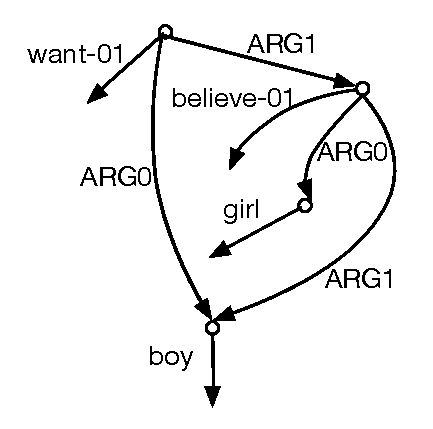
\includegraphics{./amr_example.eps}
}
\caption{An example of AMR graph representing the meaning of: ``The boy wants the girl to believe him"}
\label{fig:amr-example}
\vspace{-1em}
\end{center}
\end{figure}
The task of AMR graph parsing 
is to map natural language strings to AMR semantic graphs. \namecite{flanigan2014discriminative} propose a two-stage parsing
algorithm which first maps meaningful continuous spans on the string side to concept fragments
on the graph side, and then in the second stage adds additional edges to
make all these fragments connected. Concept identification \cite{flanigan2014discriminative,pourdamghanialigning} can be considered as an important first step to
relate components of the string to components in the graph.


Hyperedge replacement grammar (HRG) is a context-free rewriting formalism for generating graphs~\cite{drewes+al:1997}. 
Its synchronous counterpart, SHRG, can be used for transforming a graph from/to another structured representation such as a string
or tree structure. HRG has great potential for applications in natural language understanding and generation,
and also semantics-based machine translation. 


Learning SHRG rules 
from fixed string-to-graph alignments is a similar problem to extracting machine translation rules from fixed word
alignments, where we wish to automatically learn the best granularity for the rules with which to analyze each
sentence. \namecite{chung-cl14} present an MCMC sampling schedule to learn Hiero-style SCFG rules \cite{ChiangCL} by sampling 
tree fragments from phrase decomposition forests, which represent all possible
rules that are consistent with a set of fixed word alignments, making use of the property that each SCFG rule in the 
derivation is in essence the 
decomposition of a larger phrase pair into smaller ones.


\namecite{peng2015conll} have presented an MCMC algorithm to sample a special symbol-refined SHRG from aligned sentence-AMR pairs. They first construct {\bf fragment decomposition forest} representing possible derivations
of sentence-AMR pairs. Then they use MCMC algorithms to sample on derivation from the forest structure. The collection of rules from each derivation form the sampled SHRG. 


Using the sampled SHRG, \namecite{peng2015conll} have used Earley algorithm with cube pruning for decoding. A few simple local features have been used 
in their generative decoder. Although they have reported competitive results using a graph-grammar-based approach, there are some techniques that might be helpful to improve the system.


In this chapter, we first introduce the system framework of~\namecite{peng2015conll}.
Then I will propose some possible directions of improving their results. 
\section{Hyperedge Replacement Grammar}
\begin{figure}
\begin{center}
\resizebox{\linewidth}{!}{
\scalebox{0.45}{
    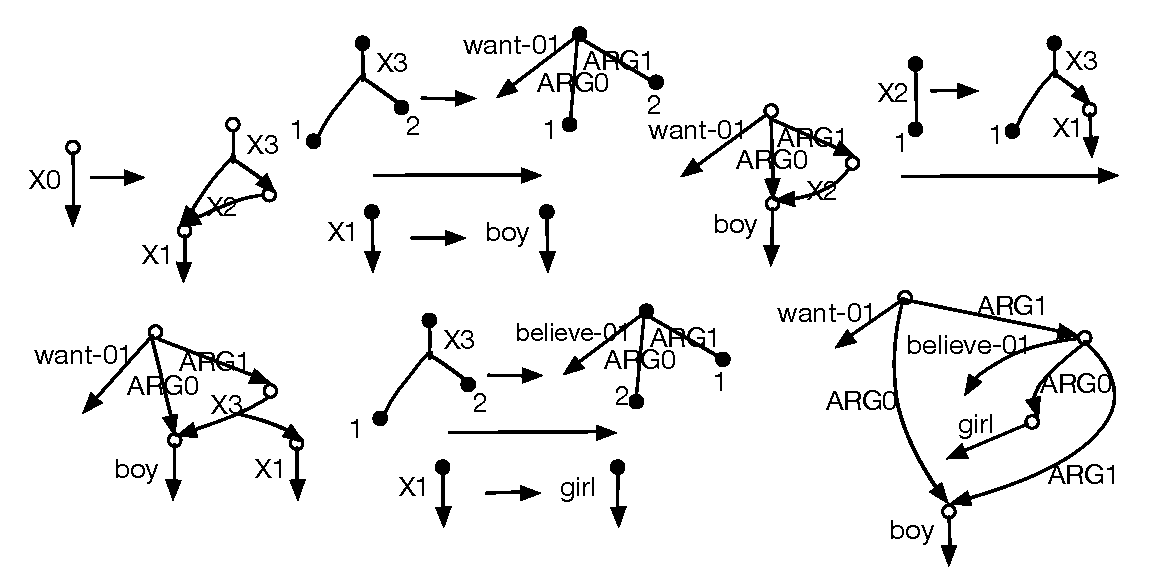
\includegraphics{./HRG.eps}
}
}
\caption{The series of HRG rules applied to derive the AMR graph of ``The boy wants the girl to believe him". The first rule is directly shown. The other HRG rules
are either above or below each right arrow. The white circle shows the root of each hyperedge. The indexes in each rule show the one-to-one mapping
between the attachment nodes of l.h.s.\ nonterminal edges and the external nodes of the r.h.s.\ subgraph}
\label{fig:hrg-example}
\vspace{-1em}
\end{center}
\end{figure}
Hyperedge replacement grammar (HRG) is a context-free rewriting formalism for graph generation \cite{drewes+al:1997}. 
HRG is like CFG in that it rewrites nonterminals independently.
While CFG generates natural language strings by successively rewriting nonterminal tokens, the nonterminals in 
HRG are hyperedges, and each rewriting step in HRG replaces a hyperedge nonterminal with a subgraph instead of a span of a string.
\subsection{Definitions}
In this paper we only use edge-labeled graphs
because using both node and edge labels complicates the definitions in our HRG-based approach. Figure~\ref{fig:hrg-example} 
shows a series of HRG rules applied to derive the AMR graph shown in Figure~\ref{fig:amr-example}.


The rewriting mechanism replaces a nonterminal 
hyperedge with the graph fragment specified by a production's
righthand side (r.h.s),\ attaching each external node of the 
r.h.s.\ to the corresponding attachment node of the lefthand side.
Take Figure~\ref{fig:hrg-example} as an example. 
Starting from our initial hypergraph with one edge 
labeled with the start symbol $``X0"$, we select one edge with nonterminal label in our current hypergraph, 
and rewrite it using a rule in our HRG\@. The first rule rewrites
the start symbol with a subgraph shown on the r.h.s..\ We continue the rewriting steps 
until there are no more nonterminal-labeled edges. 


The synchronous counterpart of HRG can be used for transforming graphs from/to another form of natural language representation. 
Productions have the form $(A\to \langle S, R\rangle , \sim)$, where $A \in N$ and $S$ and $R$ are called the source and the target and at least one of them should be
hypergraphs over $N\cup T$. $\sim$ is a bijection linking nonterminals mentions in $S$ and $R$.
In our case, the source side is a CFG and the target side is an HRG\@. Given such a synchronous grammar and a string as input, we can 
parse the string with the CFG side and then derive the counterpart graph by deduction from the derivation. The benefit of 
parsing with SHRG is that the complexity is bounded by a CFG-like parsing.

\begin{figure}
\begin{center}
\resizebox{\linewidth}{!}{
\scalebox{0.55}{
    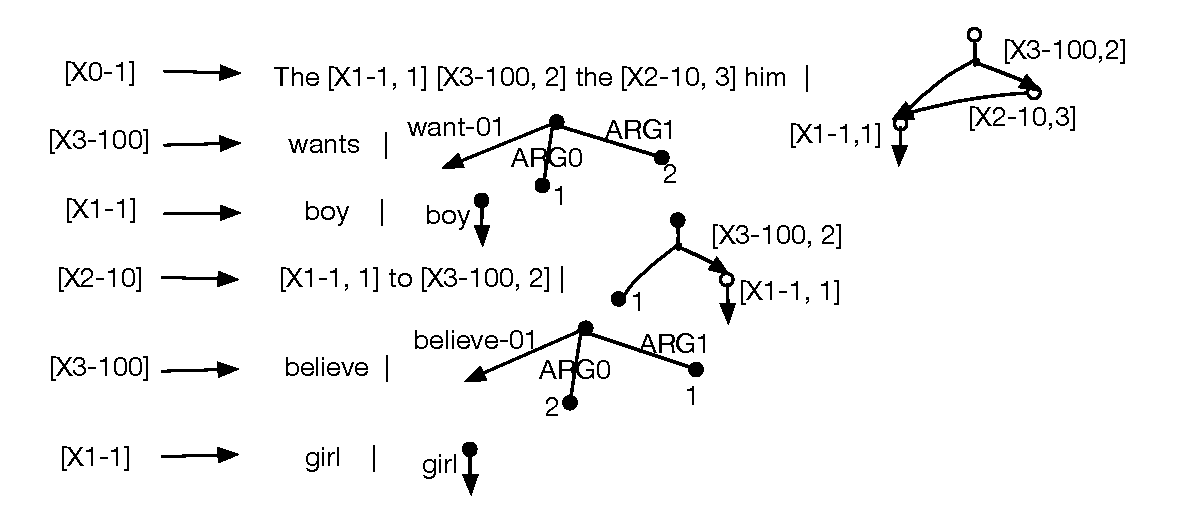
\includegraphics{./SHRGrules.eps}
}
}
\caption{A series of symbol-refined SHRG rules used to derive the AMR graph for the sentence ``The boy wants the girl to believe him".}
\label{fig:shrg-example}
\vspace{-1em}
\end{center}
\end{figure}
\namecite{peng2015conll} have used a special symbol-refined SHRG where
edge nonterminal label has an extra binary
flag, representing whether it will have a concept edge in the
final rewriting result, for each external node. The basic intuition is to explicitly enforce the one concept edge constraint
in each nonterminal so that no additional concept edge is introduced after applying each rule. The graph
derived from this type of SHRG is guaranteed to have exactly one concept edge at each node.


Figure~\ref{fig:shrg-example} shows one example of our symbol-refined SHRG\@.
For each nonterminal $Xi$-$b_1\cdots b_i$, $i$ defines the type of the nonterminal, while
each $b_i$ indicates whether the $i$-th external node will have a concept edge
in the rewriting result.\footnote{$X0$-1 is different as $X0$ is the start symbol of type one and should always have a concept edge at the root}
The second rule, for example, rewrites nonterminal $X3$-100 with {\em wants} on the string side and a hypergraph with three external nodes where 
the root has a concept edge {\em :want-01} as the first binary flag 1 indicates, while the other two external nodes do not with the binary flag 0. 
This guarantees that when we integrate the r.h.s.\ into
another graph, it will introduce the concept edge {\em :want-01} to the first fusing position
and no concept edge to the next two.
\section{Sampling SHRG from forests}
The fragment decomposition forest provides a compact representation of all possible SHRG rules that are consistent with a fixed string-to-graph 
alignment. 
We first build a forest representation of possible derivations and then use an MCMC algorithm to
sample tree fragments from this forest representing each rule in the derivation.

\subsection{Fragment Decomposition Forest}
We leave out the details of the forest construction procedure, which is introduced in~\namecite{peng2015conll}. The bottom-up construction procedure starts from the 
smallest phrase-fragment pairs, which are the sentence-AMR alignments.
Then we keeping composing larger phrase-fragment pairs until the root of the forest is reached, which is the complete sentence-AMR pair.
To further reduce the complexity of the forest construction procedure, \namecite{peng2015conll} have also deterministically attached each unaligned relation edge to one of the identified concept 
fragments it connects to.
%Figure~\ref{fig:decompose-example} shows the procedure of building the fragment decomposition forest 
%for the sentence ``The boy wants the girl to believe him".
\subsection{MCMC sampling}
Sampling methods have been used to learn Tree Substitution Grammar (TSG) rules from derivation trees \cite{cohn-2009-inducing,PostGildea-acl09} for TSG learning. 
The basic intuition is to automatically learn the best granularity for the rules
with which to analyze our data. Our problem, however, is different in that we need to
sample rules from a compact forest representation. We need to sample one tree from the forest, and then
sample one derivation from this tree structure, where each tree fragment represents one rule in the derivation. Sampling tree fragments from forests is described in detail in \namecite{chung-cl14} and \namecite{peng-gildea-emnlp14}.


We formulate
the rule sampling procedure with two types of variables: an edge variable $e_n$ representing which incoming hyperedge is chosen at a given node $n$ in the 
forest (allowing us to sample one tree from a forest) and a cut variable $z_n$ representing whether node $n$ in forest is a boundary between two SHRG rules
or is internal to an SHRG rule (allowing us to sample rules from a tree). 
Figure~\ref{fig:sampled-example} shows one sampled derivation from the forest.
We have sampled one tree from the forest using the edge variables.  We also have a 0-1 variable at each node in this tree where 0 represents the 
current node is internal to an SHRG rule, while 1 represents the current node is the boundary of two SHRG rules.
\begin{figure}
\begin{center}
\scalebox{0.50}{
    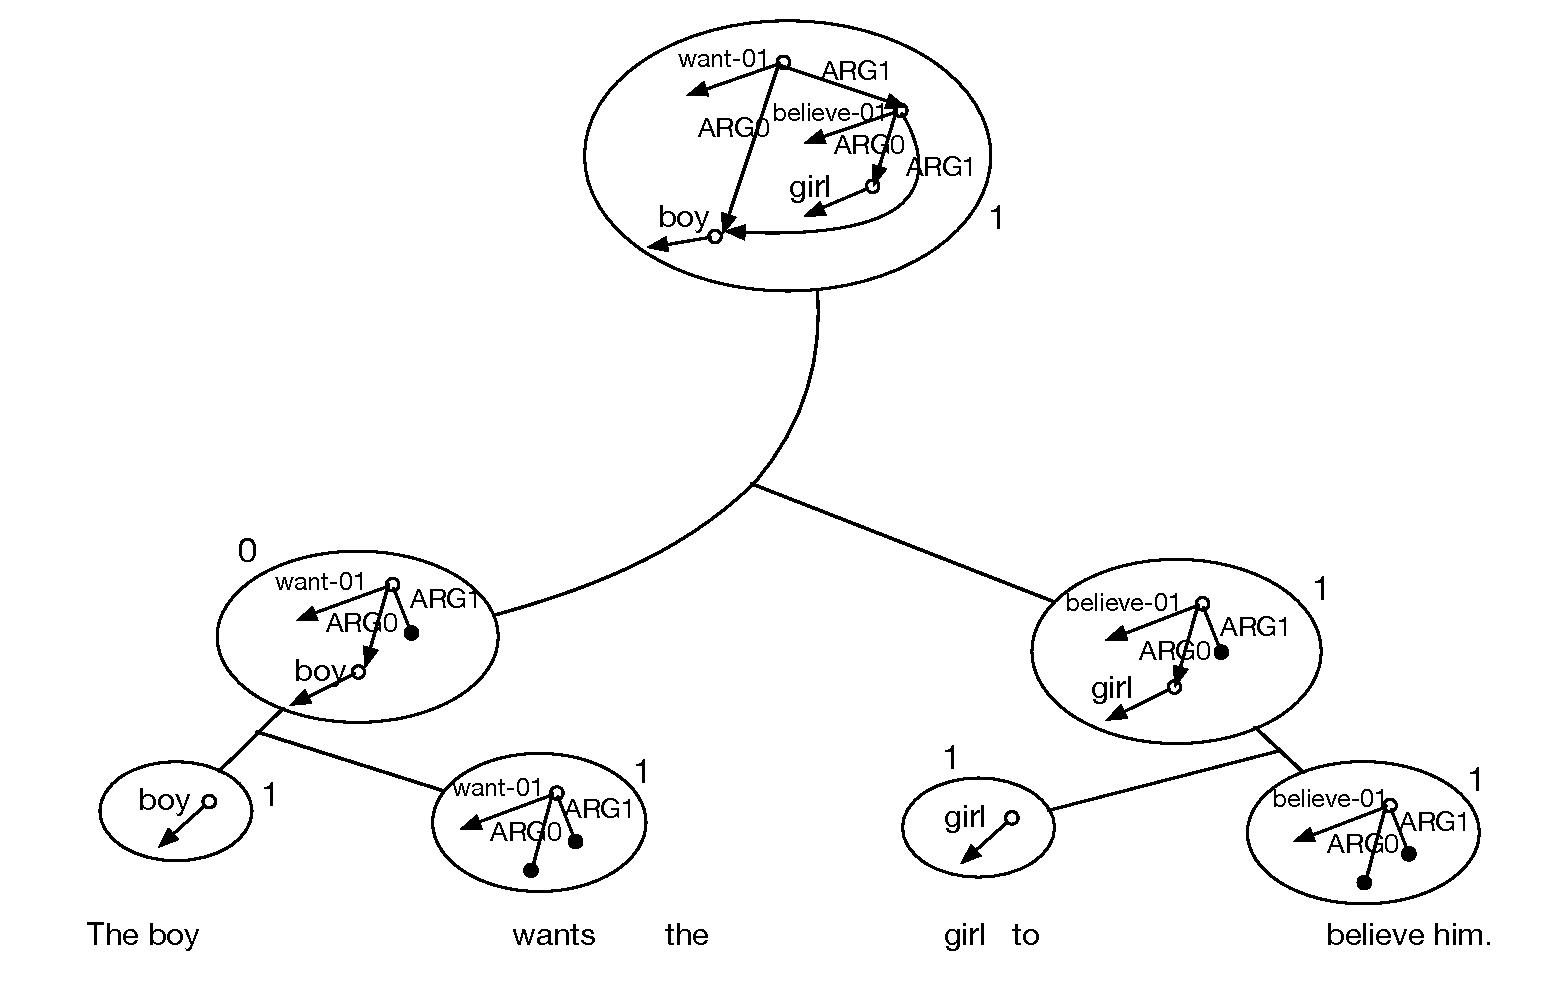
\includegraphics{./Sampled.eps}
}
\caption{The sampled derivation for the (sentence, AMR graph) pair for ``The boy wants the girl to believe him"}
\label{fig:sampled-example}
\end{center}
\end{figure}

Let all the edge variables form the random vector $Y$ and all the cut variables form the random vector $Z$. Given an assignment $y$ to the edge variables and assignment $z$ to the cut variables, our desired distribution is proportional to the product of weights of the rules specified by the assignment:
\begin{equation}\label{eq:tsg}
 P_t(Y=y, Z=z) \propto \prod_{r \in \tau(y, z)} w(r) 
\end{equation}
where $\tau(y, z)$ is the set of rules identified by the assignment and $w(r)$ is the weight for each individual rule. We use a generative model based on a Dirichlet Process (DP) defined over composed rules. We draw a distribution $G$ over rules from a DP, and then rules from $G$. 
\begin{align*}
G\mid \alpha,P_0\sim& Dir(\alpha,P_0)\\
r\mid G\sim& G
\end{align*}

We define two rules to have the same {\bf rule type} if they have the same string and hypergraph
representation (including order of external nodes) on the r.h.s..
For the base distribution $P_0$, we use a uniform distribution where all rules of the same size have equal probability.
By marginalizing out $G$ we get a simple posterior distribution over rules which can be derived using the Chinese Restaurant Process (CRP). 


For the base distribution $P_0$, we use a uniform distribution where all rules of the same size have equal probability:
\begin{equation}
P_0 (r) = V_f^{-|r_f|} V_e^{-|r_e|}
\end{equation}
where $V_f$ and $V_e$ are the vocabulary sizes of the source language and the target language, and $|r_f|$ and $|r_e|$ are the lengths of the source side and target side of rule $r$. By marginalizing out $G$ we get a simple posterior distribution over rules which can be described using the Chinese Restaurant Process (CRP). For this
analogy, we imagine a restaurant has infinite number of tables that represent rule types and customers that represent translation rule
instances. Each customer enters the restaurant and chooses a table to sit at. Let $z_i$ be the table chosen by the $i$-th customer, then the customer chooses a table $k$ either having been seated or a new table with probability:
\begin{equation}
\label{eq:CRP}
P(z_i = k| z_{-i}) = \begin{cases} \frac{n_k}{i-1+\alpha} & 1 \leq k \leq K  \\ \frac{\alpha}{i-1+\alpha} & k = K+1\end{cases}
\end{equation}
where $z_{-i}$ is the current seating arrangement, $n_k$ is the number of customers at the table $k$, 
$K$ is the total number of occupied tables. If the customer sits at a new table, the new table will be 
assigned a rule label $r$ with probability $P_0(r)$. We can see from Equation~\ref{eq:CRP} that the 
only history related to the current table assignment is the counts in $z_{-i}$. Therefore, we define a 
table of counts $N=\{N_C\}_{C\in I}$ which memorizes different categories of counts in $z_{-i}$. $I$ 
is an index set for different categories of counts. Each $N_C$ is a vector of counts for category $C$. We have $P(r_i = r| z_{-i})= P(r_i = r| N)$. If we marginalize over tables labeled with the same rule, 
we get the following probability over rule $r$ given the previous count table $N$:
\begin{equation}
P(r_i = r| N) = \frac{N_R(r) + \alpha P_0 (r)}{n + \alpha }
\end{equation}
here in the case of DP, $I=\{R\}$, where $R$ is the index for the category of rule counts. $N_R(r)$ is the number of times that rule $r$ has been observed in $z_{-i}$, $n=\sum_r N_R(r)$ is the total number of rules observed.


We define a 
table of counts $N=\{N_C\}_{C\in I}$ which memorizes different categories of counts in 
the previous assignments, where $I$
is an index set for different categories of counts. Each $N_C$ is a vector of counts for category $C$. 
We have the following probability over rule $r$ given the previous count table $N$:
\begin{equation}
P(r_i = r| N) = \frac{N_R(r) + \alpha P_0 (r)}{n + \alpha }
\end{equation}
here in the case of DP, $I=\{R\}$, where $R$ is the index for the category of rule counts.


We use the {\em top-down} sampling algorithm of \namecite{chung-cl14} which samples cut and edge variables from top down and one at a time.
For each node $n$, we denote the composed rule type
that we get when we set the cut of node $n$ to 0 as $r_1$ and the two 
split rule types that we get when we set the cut to 1 as $r_2, r_3$. We sample the cut value $z_i$ of the 
current node according to the posterior probability:
\begin{equation}
\label{eq:cut}
\resizebox{.88\hsize}{!}{$\displaystyle
P(z_i = z| N) = 
\begin{cases} 
\frac{ P (r_1| N) }{P (r_1|N) + P (r_2| N) P (r_3| N') } &\mbox{if } z = 0 \\ 
\frac{ P (r_2| N) P (r_3| N') }{P (r_1| N)+ P (r_2| N) P (r_3| N') } &\mbox{otherwise}
\end{cases}$}
\end{equation}
where the posterior probability $P(r_i|N)$ is according to a DP, 
and $N, N'$ are tables of 
counts. In the case of DP, $N, N'$ differ only in the rule counts of $r_2$, where $N'_R(r_2)= 
N_R(r_2)+1$.


As for edge variables $e_i$, we refer to the set of composed rules turned on below $n$ including the 
composed rule fragments having $n$ as an internal or root node as $\{r_1,\ldots,r_m\}$. We have the 
following posterior probability over the edge variable $e_i$:
\begin{equation}
\resizebox{.88\hsize}{!}{$\displaystyle
P(e_i = e| N) \propto \prod_{i=1}^m P(r_i| N^{i-1}) \prod_{v \in \tau(e)\cap \mbox{in}(n)} \mbox{deg}(v)
$}
\end{equation}
where $\mbox{deg}(v)$ is the number of incoming edges for node $v$, 
$\mbox{in}(n)$ is the set of nodes 
in all subtrees under $n$, and $\tau(e)$ is the tree specified when we set $e_i = e$. $N^0$ to $N^m$ 
are tables of counts where $N^0 = N$, $N^i_R(r_i) = N^{i-1}_R(r_i) + 1$ in the case of DP.


We sample from top-down, sample cut, sample edge and one variable at a time. When we have sampled one tree from the forest
and the boundaries of tree fragments, we have sampled one derivation which represents the series of rules applied to derive
the sentence-AMR pair. We should note that this algorithm is not Gibbs sampling because of the density term $\mbox{deg}(v)$.
\section{Decoding}
We use Earley algorithm with cube-pruning \cite{ChiangCL} for the string-to-AMR parsing. 
For each synchronous rule with $N$ nonterminals on its l.h.s., we build an $N+1$ dimensional cube and generate top $K$ candidates. 
Out of all the hypotheses generated by all satisfied rules within each span $(i,j)$,we keep at most $K$ candidates for this span.
Our glue rules will create a pseudo $R/ROOT$ concept and use $ARG$s relations to connect
disconnected components to make a connected graph.


We use the following local features:
\begin{enumerate}\footnotesize
    \item StringToGraphProbability: the probability of a hypergraph given the input string
    \item RuleCount: number of rules used to compose the AMR graph
    \item RuleEdgeCount: the number of edges in the r.h.s.\ hypergraph 
    \item EdgeType: the type of the l.h.s.\ nonterminal. For rules with same source side tokens, we prefer rules with smaller edge types.
    \item AllNonTerminalPunish: one for rules which only have non-terminals on the source side.
    \item GlueCount: one for glue rules.  
\end{enumerate}

\section{Proposed methods}
\subsection{Categorize AMR graphs with limited types}
One problem with AMR graph parsing is the sparsity of the word vocabulary and types of concepts. Unknown content words appeared in the training data, if unaligned, could
break up the structure of the derivation when decode from bottom up. Even if we can retrieve the content words using external resources, it is hard to assign a new weight to these lexical rules.
Assigning uniform weight to the retrieved rules would be harmful because different types of words should have different relative importance.


It would be helpful to deal with unknown words if we already have unknown words in the training data and we can learn the probabilities for these unknown words.
One strategy would be to use relative frequency of words: if a word appears fewer than a certain frequency threshold, we can reduce the word to its POS tag or a special \textit{UNKNOWN} token. We can also flip low-frequency words into \textit{UNKNOWN} tokens or its POS tag with 
probability $\frac{1}{2}$.


Another problem with AMR parsing is the argument structures for the predicates. Usually the types of arguments for each predicate does not always appear in the training data.
However, during the decoding procedure, the decoder would prefer rules that have the predicate in them, even though the argument types are totally wrong.
If we can categorize the predicates into different types, then the argument types for each category would be less sparse then the specific word.
For example, we can reduce \textit{give-01} and \textit{bring-01} to \textit{PRED-01}, then we can combine the argument types of \textit{give-01} and \textit{bring-01} 
to build the argument types for \textit{PRED-01}. We can also categorize special nouns or adjectives which are mapped to predicate structure. For example, some nouns that end with "-ion" or "-er".


With a smaller categories, our sampling algorithm would also benefit from the smaller number of rule types and larger frequency of each type. With the larger frequency for each category, we can also rule out some alignment errors which are 
more likely to be introduced when the word frequency is low.


Another useful resources is the roles and verbalization lists from isi.\footnote{http://amr.isi.edu/download.html} These lists are used during
the annotation of AMR datasets and are therefore provide important guidelines on how to categorize words on those lists.


After we have categorized the words and concepts, we need additional postprocessing to map the reduced category to its real concept label. This
procedure is very easy to deal with since we have the alignment from the original word to the category and we can build a map between words and their most frequently mapped concept.
\subsection{Forced decoding}
The generative decoding model has a few limitations: 1. the features are very simple and no global feature is included. 2. All the weights of the features are
set by hand, which suffers from the limit of huge space of combination of the weights.
One way to deal with these limitations is to use a feature-rich discriminative model. The training data is used to extract the SHRG, more specifically
rules and the count for each rule. However, the structural information of the derivation forest is not used. Using a discriminative model which
learns to search within the forest structure would make use of more structural information in our training data.


\namecite{yu-EtAl:2013:EMNLP} have proposed a structured perceptron algorithm that learns to search for derivations that generate the whole or prefixes of the 
target reference sentences for phrase-based machine translation. Beam search is used to reduce the intractable search space and each bin $B_i$ maintain a K-best list of hypotheses that covers $i$ words
on the source side. A search error happens for a certain hypothesis $d$ when its target side $e(d)$ is not a prefix of the reference $y$.


In our AMR parsing scenario, we have a derivation forest representing possible ways to compose sentence-AMR pairs. Let $<x, y>$ be a sentence-AMR pair in the training data. We can 
compare the AMR graph side to the target side sentence and each hypothesis $d$ contains a span-subgraph pair derived from a series of rule applications:
$$d = r_1 \circ r_2 \circ \cdots \circ r_{|d|}$$
where each $r_i$ is a SHRG rule and $d=(e(d), g(d))$ is a (partial) derivation whose source side $e(d)=(x_i, \cdots , x_j)$ is a span which covers 
positions $[i, j]$ and whose target side is a subgraph $g(d)$ generated so far. 


We maintain the a bin $B_{ij}$ for each span $[i, j]$. Let $sub(y)$ be all the subgraphs
of target side AMR $y$ and $good_{ij} (x, y)$ be set of partial $y$-good derivations whose graph side is a subgraph of the reference AMR graph $y$
and the sentence side covers span $[i, j]$:
$$good_{ij}(x, y)\triangleq \{d \in D(x) | g(d) \in sub(y), e(d)=(x_i, \cdots , x_j)\}$$

Conversely, we define $y$-bad partial derivations $bad_{ij}(x,y)$ as follows:
$$bad_{ij}(x, y)\triangleq \{d \in D(x) | g(d) \notin sub(y), e(d)=(x_i, \cdots , x_j)\}$$

The search using Earley algorithm proceeds as follows: use the \textit{scan} and \textit{complete} operation to find items that covers source span $[i, j]$. 
The cost for each item is scored as: 
$${\bf w} \cdot {\bf \Phi}(x, d, i, j)$$
where $d$ is the partial derivation constructed so far. $\Phi$ is the features extracted within span $[i, j]$ and the partial derivation $d$. We keep two separate
grammars to derive $good_{ij}(x, y)$ and $bad_{ij}(x, y)$. The $good_{ij}(x, y)$ is constructed by searching along the constructed forest, that is, follow the supervision of
the composition of the sentence-AMR pair and therefore always derives a partial $y$-good derivations. $bad_{ij}(x, y)$ is constructed by searching through the whole grammar, which tries to find the derivation that has the greatest
global score. Assume we have $K$ items at each bin, we gradually build up each bin using recursion:
$$B_0 = \{ \emptyset \}$$
$$B_{ij} = \textbf{top}^K (good_{ij}(x,y)) \cap \textbf{top}^K (bad_{ij}(x,y))$$
where $\textbf{top}^K$ is an operator which computes the top $K$ items of a stack according to the scoring function.


The perceptron works by adjusting the weights whenever search error happens and different variations of the perceptron algorithm make update
at different points. The standard perceptron algorithm works by decoding the whole sentence first and update if the predication for the whole
sentence does not match the reference. This update has the problem that in cases where search error happens at a very early step and there is
no $y$-good item left in the bin. There is little point in continuing the search and update the parameters afterwards.


Early update is a special case of violation-fixing perceptron which stops decoding whenever the gold derivation falls off the beam. It makes update on the partial derivation so far and 
move on to the next training example when the update finishes. As we don't actually have the gold derivation, we replace it with
the item in $good_{ij}(x,y)$ that has the largest score.
$$d_{ij}^{+} \triangleq {\bf \argmax}_{d\in good_{ij}(x,y)} {\bf w}\cdot \Phi(x, d, i, j)$$
$$d_{ij}^{-} \triangleq {\bf \argmax}_{d\in bad_{ij}(x,y)} {\bf w}\cdot \Phi(x, d, i, j)$$
$${\bf w} \leftarrow {\bf w} + \triangle \Phi(x, d_{ij}^{+}, d_{ij}^{-}, i, j)$$
where $\triangle \Phi(x, d, d', i, j) \triangleq \Phi(x, d, i, j) - \Phi(x, d', i, j)$ is the notation for the difference of feature vectors.


In practice, there are exponentially many $y$-good derivations for each sentence-AMR pair and our goal is to make sure the $y$-good derivation would succeed in the end. 
It is possible that in a certain span $[i,j]$ all $y$-good derivations fall off the bin, but search can still succeed from other spans.
Therefore, we will continue the search through all possible spans until we reach the condition that there is no hope of finding another 
$y$-good derivation.


Another way of doing parameter update is to use \textit{max-violation} proposed by Huang et al. (2012). The basic idea is to update at the
point where the mistake is the biggest. More specifically, the update step is:
$$(ij)^{*} \triangleq {\argmin}_{ij} {\bf w} \cdot \triangle \Phi(x, d_{ij}^{+}, d_{ij}^{-}, i, j)$$
$${\bf w} \leftarrow {\bf w} + \triangle \Phi(x, d_{(ij)^*}^{+}, d_{(ij)^*}^{-}, i, j)$$

\subsection{Dependency tree to AMR graph}
It is well motivated to use dependency tree information because of dependency tree and AMR graphs are linguistically similar to each other.
As we can also use the left-to-right order of the dependency tree, therefore, instead of extracting a synchronous grammar for sentence-AMR pairs, we can
extract a synchronous grammar for dependency-AMR pairs.
In this synchronous grammar, the dependency side would be a subtree instead of a span. Such kind of grammar would also provide more useful features during the decoding procedure.
\section{Schedule}
I will start this project from 2016 Fall. AMR graph categorization should be done during the first month. I will also start implementing forced decoding for AMR parsing during the same time.
The implementation should be done before November. The target of this project is NAACL 2017. Tuning the performance should be done before the deadline.
\section{Conclusion}
We have presented an MCMC algorithm for sampling SCFG rules from derivation forests constructed from aligned sentence-AMR pairs.
With the extracted grammar, we used Earley algorithm with cubing pruning to decode each sentence. To overcome the limitations of
simple local features and the hand-tuned weights for each feature, we propose a feature-rich discriminative model using forced decoding to
include rich global features and adjust the weights using perceptron update.
We have also proposed a categorization technique which categorize words into types to deal with the sparsity of grammar. 
As dependency trees and AMR graphs are linguistically similar, we also propose to learn a synchronous grammar where the sentence side is replaced with a dependency tree structure.
